\section{Our Implementation }\label{sec:impl}

%\begin{figure*}[h]
%  \centering
%  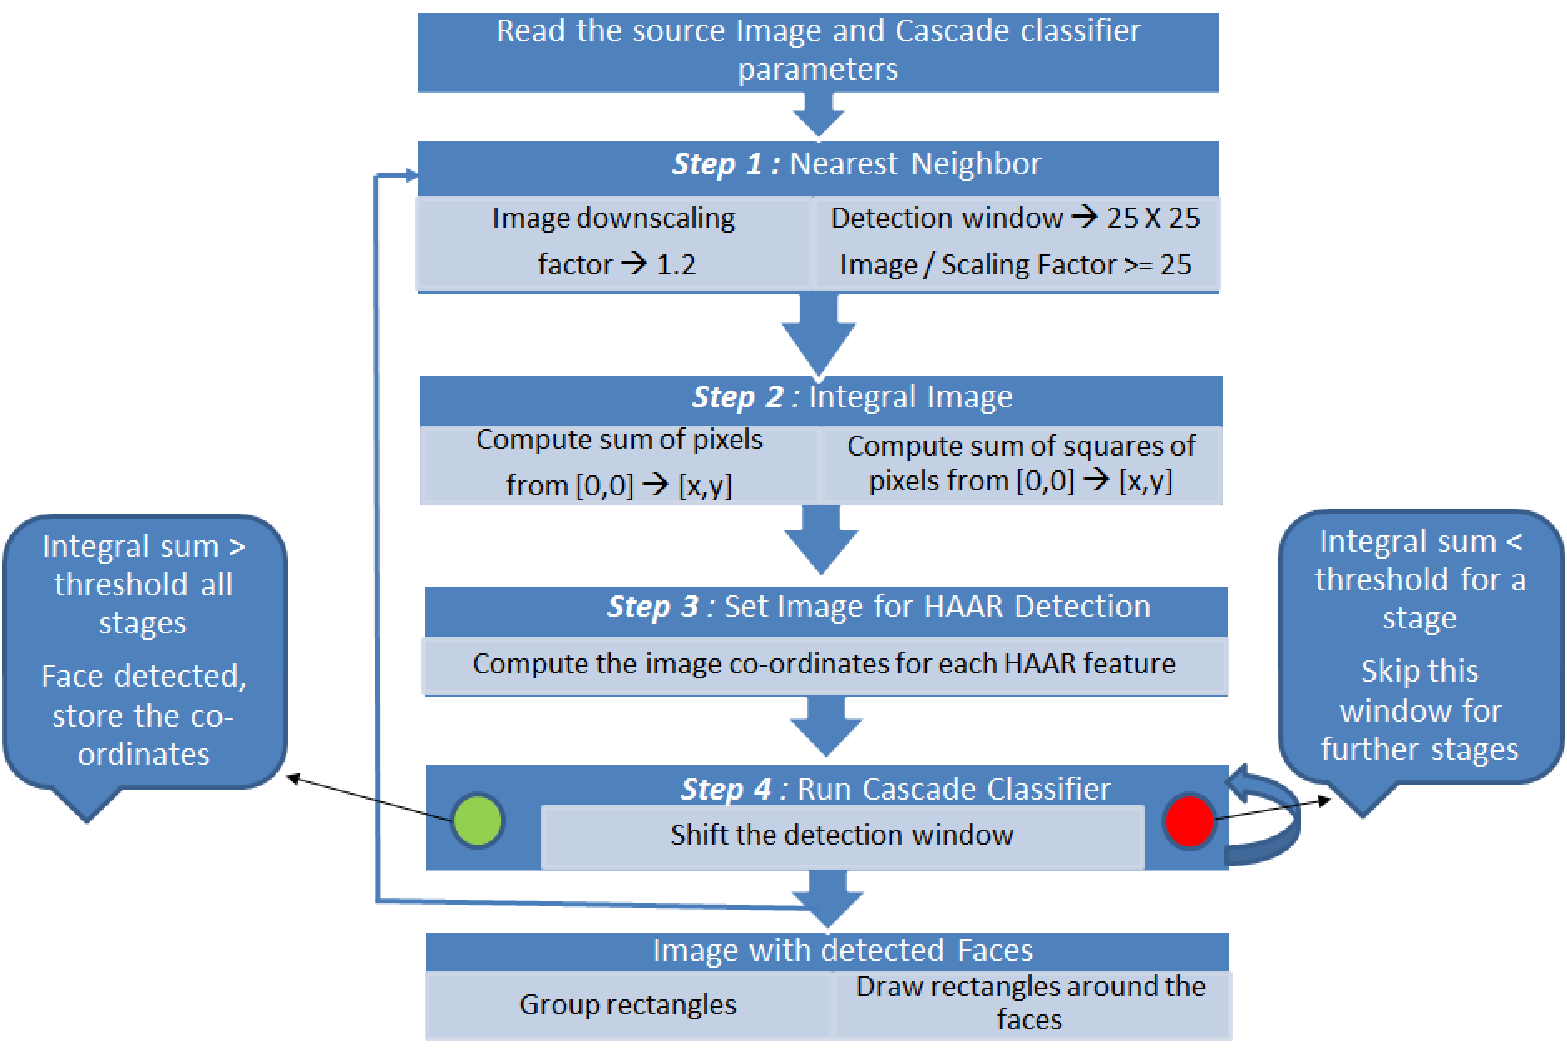
\includegraphics[width=0.75\linewidth]{figs/flow_crop.pdf}
%  \caption{Face detection implementation flow }
%  \label{fig:flow}
%\end{figure*}


Figure~\ref{fig:flow} shows the overall flow of the data. First, we read
the input image and the cascade classifier parameters into CPU side data structures. 
Then compute the downscaled image and perform the integral sum in step 1 and 2 respectively. 
Next, we determine the downscaled image co-ordinates required for each HAAR features in step three. 
These are the relative positions of each HAAR rectangle boundaries in a 25 x 25 window. 
For a shifted position of the detection window,\textit{(in step 4)} the shifted offset is added to get the new co-ordinates. 
In step 4, the window is processed through each stage of cascade classifier. 
For a given stage if the integral sum is less than the threshold for that stage, 
then the remaining stages are skipped for this window\textit{(no face detected in this window)}. 
If the integral sum exceeds the threshold limit of a stage, in all the stages, then it is qualified as a face. 
In that case, the window position and image scale are stored. Once window is processed as above, 
it shifted by 1 pixel and then passed through step 4 for face detection. 
This process is continued until the total image is scanned at that particular scale. 
Then the whole process is repeated by downscaling the image in step 1 through face detection in step 4. The input image runs through this series of steps from 1 through 4 until its downscaled to the size of detection window\textit{(here, 25 X 25)}. 
Finally, we have all the window positions and the scale at which they face detected. The faces 
are indicated in the final image with a rectangle around them. If two or more faces overlap in a window 
they are taken care by the 'Group rectangles' function. 

In this project, we considered the sections in the algorithm shown in
Figure~\ref{fig:flow} that
can be parallelized, wrote kernels for each of them in CUDA
and offloaded them to execute on GPU. The sections that
can be parallelized are Nearest Neighbor, Integral Image and Scan Window Processing
\textit{(referred to 'Set Image for HAAR Detection' \& 'Run Cascade Classifier' together)}
 which are explained below.
\vspace{0.1in}
\begin{itemize}

\item \textbf{Nearest Neighbor}
We have fixed size window (25x25) for each feature. But the face in the image can be of any scale. 
To make the face detection scale  invariant, we have used pyramid of images that contain downscaled versions of the original image. 
Since each pixel can be processed separately, 
we produced image pyramid on GPU. Example of an image pyramid is shown in Figure~\ref{fig:scale}.

\begin{figure}[h]
  \centering
  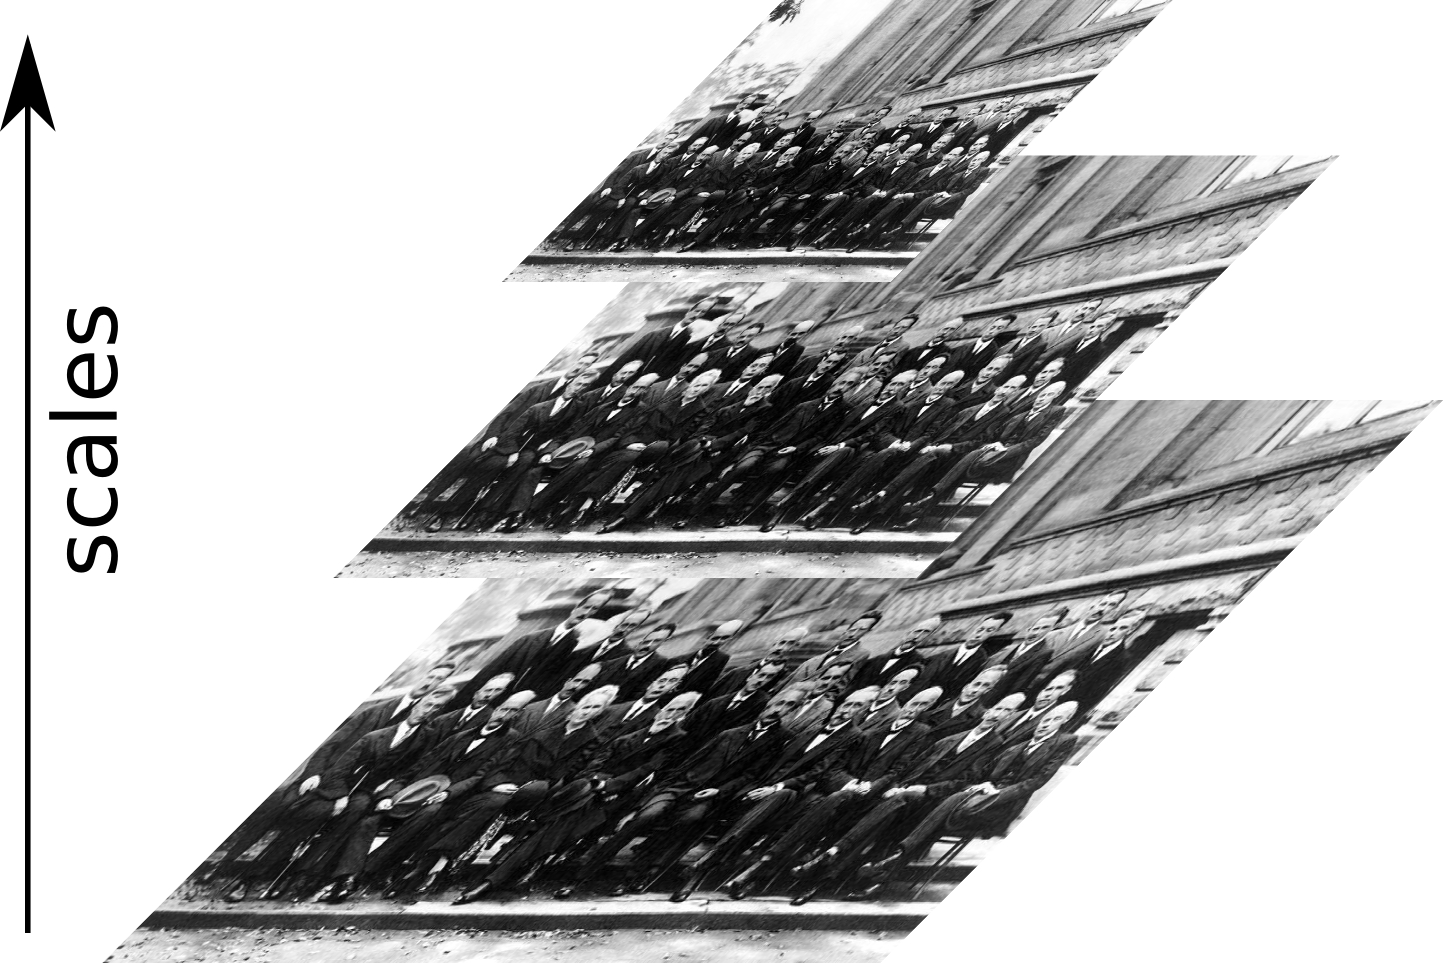
\includegraphics[width=0.65\linewidth]{figs/scale.jpg}
  \vspace{0.05in}
  \caption{Image Pyramid \textnormal{\small }  }
  \label{fig:scale}
\end{figure}

\vspace{0.1in}
\item \textbf{Integral Image Calculation}
Integral image calculation is essentially 2-dimensional inclusive scan. To avoid data dependency of image integral calculation, we adopted the 
algorithm of first 
row integral and then column integral calculation.

\vspace{0.1in}
\item \textbf{Scan Window Processing}
Since each 25x25 image sub-window has to pass through all the features, each thread in the GPU 
can perform parallely on a sub-window. But the design of cascade classifier is such that after 
each stage the doubtless non-face scan sub-windows are eliminated as much as possible. Hence we 
considered each stage separately and sequentially, and executed group of stages as a different kernel.
Figure~\ref{fig:scan} show the principle of using parallel scan windows. 

\begin{figure}[h]
  \centering
  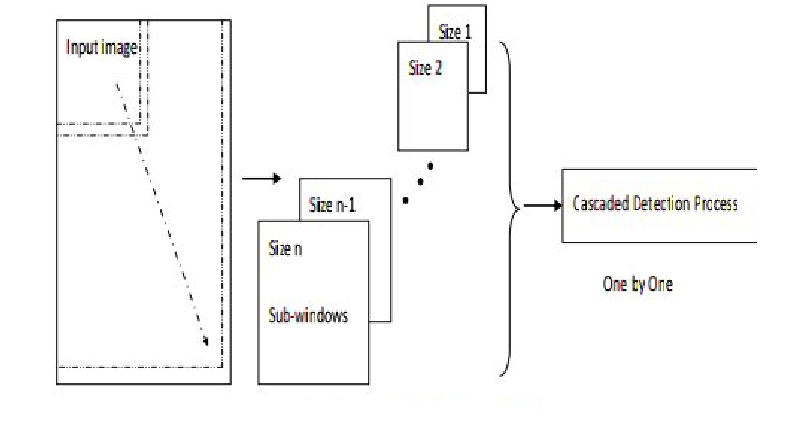
\includegraphics[width=\linewidth]{figs/scan_crop.pdf}
  \caption{Scan Window Processing \textnormal{\small }  }
  \label{fig:scan}
\end{figure}



\end{itemize}

